% !TEX encoding = UTF-8 Unicode
\documentclass[a4paper, twocolumn]{article}

\usepackage{color}
\usepackage{url}
\usepackage[T2A]{fontenc} % enable Cyrillic fonts
\usepackage[utf8]{inputenc} % make weird characters work
\usepackage{graphicx}

\usepackage[english,serbian]{babel}

\usepackage[unicode]{hyperref}
\hypersetup{colorlinks,citecolor=green,filecolor=green,linkcolor=blue,urlcolor=blue}

\usepackage{listings}
\usepackage[ruled,vlined,croatian,onelanguage]{algorithm2e}

\SetKwInput{KwInput}{Ulaz}                % Set the Input
\SetKwInput{KwOutput}{Izlaz}
%SetKw{KwResult}{Rezultat}
%\SetKw{}{radi}
\definecolor{mygreen}{rgb}{0,0.6,0}
\definecolor{mygray}{rgb}{0.5,0.5,0.5}
\definecolor{mymauve}{rgb}{0.58,0,0.82}

\lstset{ 
  backgroundcolor=\color{white},   % choose the background color; you must add \usepackage{color} or \usepackage{xcolor}; should come as last argument
  basicstyle=\footnotesize,        % the size of the fonts that are used for the code
  breakatwhitespace=false,         % sets if automatic breaks should only happen at whitespace
  breaklines=true,                 % sets automatic line breaking
  captionpos=b,                    % sets the caption-position to bottom
  commentstyle=\color{mygreen},    % comment style
  deletekeywords={...},            % if you want to delete keywords from the given language
  escapeinside={\%*}{*)},          % if you want to add LaTeX within your code
  extendedchars=true,              % lets you use non-ASCII characters; for 8-bits encodings only, does not work with UTF-8
  firstnumber=1000,                % start line enumeration with line 1000
  frame=single,	                   % adds a frame around the code
  keepspaces=true,                 % keeps spaces in text, useful for keeping indentation of code (possibly needs columns=flexible)
  keywordstyle=\color{blue},       % keyword style
  language=Python,                 % the language of the code
  morekeywords={*,...},            % if you want to add more keywords to the set
  numbers=left,                    % where to put the line-numbers; possible values are (none, left, right)
  numbersep=5pt,                   % how far the line-numbers are from the code
  numberstyle=\tiny\color{mygray}, % the style that is used for the line-numbers
  rulecolor=\color{black},         % if not set, the frame-color may be changed on line-breaks within not-black text (e.g. comments (green here))
  showspaces=false,                % show spaces everywhere adding particular underscores; it overrides 'showstringspaces'
  showstringspaces=false,          % underline spaces within strings only
  showtabs=false,                  % show tabs within strings adding particular underscores
  stepnumber=2,                    % the step between two line-numbers. If it's 1, each line will be numbered
  stringstyle=\color{mymauve},     % string literal style
  tabsize=2,	                   % sets default tabsize to 2 spaces
  title=\lstname                   % show the filename of files included with \lstinputlisting; also try caption instead of title
}

\begin{document}
  


\title{Generički algoritam klasterovanja zasnovan na optimizaciji rojem čestica\\
\small{XLVIII Međunarodni simpozijum\\ o operacionim istraživanjima}}

\author{Denis Aličić
\\denis\char`_alicic@matf.bg.ac.rs\\}

\maketitle

\abstract{
U ovom radu je opisan razvijeni algoritam klasterovanja zasnovan na optimaciji rojem čestica \cite{pso}. Algoritam je zasnovan na centroidima, slično algoritmu K sredina. Najvažniji parametar algoritma je funkcija kvaliteta klasterovanja koja se optimizuje i time određuje tip klastera. Jedna čestica predstavlja niz centroida dužine k, zadate kao maksimalan broj klastera.
U svakoj iteraciji algoritma se svakoj instanci iz skupa podataka dodeli klaster na osnovu najbližeg centroida. Funkcija udaljenosti se takođe prosleđuje algoritmu i od nje zavisi oblik klastera. Zatim se primenjuje funkcija kvaliteta i na osnovu pozicije najbolje čestice i najbolje pozicije trenutne čestice pomeri centroid svakoj čestici u skladu sa originalnim PSO (eng.~{\em Particle swarm optimization}) algoritmom.\\  
Prikazani su eksperimenti na nekim poznatim skupovima podataka, kao i na sintetičkim podacima u dvodimenzionalnom prostoru radi vizuelizacije.

\setcounter{tocdepth}{1}
%\tableofcontents

%\newpage
\section{Uvod}
\label{sec:uvod}
Klasterovanje je jedan od najpopularnijih problema nenadgledanog učenja.
Predstavlja identifikaciju i grupisanje sličnih instanci u datom skupu podataka. Primene ovog metoda su vrlo široke.
Od zamene grupa njihovim predstavnicima zarad smanjenja broja instanci u skupu podataka, do detekcije raznorodnih tkiva na medicinskim snimcima i identifikaciji sličnih grupa korisnika društvenih mreža u svrhu oglašavanja.\\

Obzirom da za mnoge primene nije moguće jednoznačno odrediti šta je dobro klasterovanje, razvijene su različite metode klasterovanja.
Postojeći algoritmi se mogu svrstati u nekoliko kategorija u odnosu na vrstu i broj klastera koji su njihov rezultat.
Nekim metodama se zadaje ciljni broj klastera, dok drugi kao izlaz mogu dati različit broj klastera.
S druge strane, što se tiče vrste klastera koje daju kao izlaz razlikujemo: Globularne, dobro razdvojene, gustinske, hirejarhijske itd.\cite{ml_mladen}\\

Predloženi metod može u zavisnosti od njegovih parametara: funkcije sličnosti i funkcije kvaliteta, koje će biti opisane kasnije, da generiše različite vrste klastera, dok mu se kao poseban parametar zadaje maksimalan broj klastera.
Algoritam je primarno zasnovan na centroidama.

\section{Klasterovanje kao optimizacioni problem}
\label{sec:klasterovanje}
Kod problema klasifikacije, koji je vid nadgledanog učenja, postoje dobro definisane funkcije koje nam mogu reći kakav je kvalitet dobijenog modela. To su pre svega tačnost i preciznost, mada postoje još neke.\\

Klasterovanje je problem nenadgledanog učenja,
 tako da za konkretno grupisanje ne postoje jednoznačne funkcije koje nam sa sigurnošću mogu reći koliko je ono dobro. Ipak, postoje neke funkcije, definisane tokom vremena od raznih istraživača, koje nam mogu dati ocenu kvaliteta klasterovanja \cite{dunn}\cite{ch_score}.

Zanimljivo je primetiti, da iako na prvi pogled ne deluje tako, algoritam K sredina se takođe može posmatrati kao optimizacioni algoritam. Funkcija koju taj algoritam optimizuje je:

\[ \sum_{i=1}^{k}\sum_{x \in C_i} d(x, c_i)^2 \]

gde je $d$ rastojanje, najčešće euklidsko, ali može biti i neko drugo, a $c_i$ centroida i-tog klastera. 
\subsection{Funkcije evaluacije}
Slično metrikama koje se koriste za evaluaciju klasifikacionih modela, postoje funkcije koje koriste informaciju o stvarnim klasama da bi ocenile kvalitet klasterovanja. Neke od njih su:
\begin{itemize}
	\item Rand indeks
	\item Homogenost
	\item V-mera
\end{itemize}  

U realnim primenama stvarne klase nisu dostupne, tako da ove funkcije nisu korišćene niti prilikom implementacije algoritma, niti prilikom evaluacije, te ni u radu neće biti dalje razmatrane.\\

Funkcije koje su korišćene prilikom implementacija i eksperimenata su:
\begin{itemize}
	\item Davies-Bouldin indeks \ref{sec:db}
	\item Calinski-Harabasz indeks \ref{sec:ch}
\end{itemize}

Za izračunavanje ovih funkcija potrebna je informacija o centroidima klastera i dodeli klastera svakoj instanci iz skupa podataka.   

\subsubsection{Davies-Bouldin indeks}
\label{sec:db}
Metrika je zadata formulom:
\[ \frac{1}{c}\sum_{i=1}^{c}\max_{i \neq j} \left( \frac{\sigma_i + \sigma_j}{d(C_i, C_j)} \right) \]

gde je $c$ broj klastera, $\sigma$ prosečno rastojanje svih instanci jednog klastera od njegovog centroida, $d$ rastojanje, najčešće euklidsko i $C_i$ centroid i-tog klastera.

Minimizacijom ove funkcije po $C_i$ dobijamo grupe koje imaju malo rastojanje unutar istog klastera, a veliko rastojanje između različitih klastera \cite{db_index}.\\ 

Generalno, to je ideja većine ovih funkcija zasnovanih na centroidama, s tim što na različite načine kvantifikuju rastojanja unutar klastera i između različitih klastera. \\

Minimalna vrednost ove funkcije se dostiže u 0. Treba biti obazriv sa minimizacijom ove funkcije, jer metode sa mogućnošću povećavanja broja klastera, prilikom optimizacije ove mere teže tome da svaka tačka bude pojedinačni klaster.

U situaciji da postoji beskonačno instanci, deo funkcije $\frac{1}{c}$ bi težio ka nuli, onda bi i cela funkcija težila minimalnoj vrednosti.

\subsubsection{Calinski-Harabasz indeks}
\label{sec:ch}
Calinski-Harabasz indeks je nešto složeniji za izračunavanje i interpretaciju.\\
Za dati skup podataka $E$, veličine $n_E$, koji se klasteruje u $k$ klastera, vrednost indeksa je definisana kao odnos proseka disperzija klastera i disperzija unutar klastera.\\
Definisan je formulom:

\[ s = \frac{tr(B_k)}{tr(W_k)} \times \frac{n_E - k}{k - 1} \]

gde je $tr(B_k)$ trag matrice\footnote{Trag matrice predstavlja sumu elemenata na glavnoj dijagonali: $tr(A) = \sum_{i=1}^{n}a_{ii}$.} disperzije centroida klastera i $tr(W_k)$ trag matrice disperzije unutar pojedinačnog klastera.\\

Matrice se izračunavaju po formulama:

\[ B_k = \sum_{q=1}^{k} n_q(c_q - c_E)(c_q - c_E)^T \] 

\[ W_k = \sum_{q=1}^{k}\sum_{x \in C_q}(x - c_q)(x - c_q)^T \]

gde je $C_q$ skup instanci u klasteru $q$, $c_q$ centroid klastera $q$, $c_E$  centroida celog skupa instanci $E$ i $n_q$ broj instanci u klasteru $q$.\\

Što je ovaj indeks veći, to je klasterovanje bolje, centroide su udaljenije, a rastojanja unutar klastera manja.\\
Zbog načina računanja disperzije klastera, koje se izračunava kao kvadriran zbir udaljenosti instance od centroida, ovaj indeks je generalno veći za konveksne klastere, što je za algoritam koji je predstavljen u ovom radu prednost jer očekivani izlaz algoritma jesu konveksni klasteri.

\subsection{PSO algoritam}
\label{sec:algoritam}
Optimizacioni algoritam je zasnovan na optimizaciji rojem čestica \cite{pso}.
Pseudokod algoritma je prikazan na slici \ref{pseudokod}.
\begin{algorithm}
\SetAlgoLined
\KwResult{Broj klastera $k$, $k$ centroida i dodeljivanje klastera svakoj instanci}
\KwInput{Skup podataka, maksimalan broj klastera $k$, funkcija evaluacije, funkcija udaljenosti}
\KwOutput{Skup podataka sa pripadajucim klasterima, maksimum $k$ centroida}
 inicijalizuj početni roj\;
 odredi najbolju česticu\;
 \While{nije postignut kriterijum zaustavlja}{
  	\ForEach{česticu u roju}{
		Ažuriraj brzinu čestice na osnovu pozicije najbolje čestice i najbolje pozicije trenutne čestice\;
		Promeni poziciju čestice na osnovu izračunate brzine\;
		Na osnovu funkcije udaljenosti odredi pripadnost svakoj instanci skupa odgovarajućem klasteru\;
		Izračunaj funkciju evaluacije na osnovu dodeljenog klasterovanja\;
		\If{nova pozicija bolja od prethodne najbolje pozicije čestice\;}
		{ažuriraj najbolju vrednost trenutne čestice\;}
		\If{nova pozicija bolja od pozicije najbolje čestice\;}
		{ažuriraj poziciju najbolje čestice\;}
	}
 }
 \Return{klasterovanje najbolje čestice, broj klastera i njene centroide}
 
 \caption{PSO algoritam klasterovanja}
 \label{pseudokod}
\end{algorithm}

Osnovnu PSO algoritma čini jedna čestica roja. Čestice predstavljaju jedno rešenje optimizacionog problema.
Jednu česticu u algoritmu razvijenom za potrebe ovog rada predstavlja niz centroida klastera.
Centroidi klastera zajedno sa funkcijom blizine predstavljaju jedinstveno određeno rešenje problema klasterovanja. Za svaku instancu skupa nad kojim se vrši klasterovanje se određuje pripadajući klaster kao najbliži centroid koristeći funkciju daljine koja je prosleđena algoritmu kao parametar.
Od prosleđene funkcije daljine (euklidska distanca, kosinusna ili neka druga), zavisi oblik klastera.
Algoritam je generički u smislu izbora funkcije daljine i funkcije evaluacije koja se optimizuje.\\

Važan deo svakog algoritma optimizacije je njegova sposobnost pretrage širokog prostora rešenja u odnosu na postizanje lokalnog optimuma u nekoj manjoj oblasti. Kod PSO algoritma ovaj problem je rešen korišćenjem dva parametra koji se odnose na kognitivnu i sociološku komponentu.
Kognitivna komponenta čestice daje značajnost njenoj najboljoj poziciji, dok se sociološka komponenta odnosi na najbolju poziciju celog roja.
Menjanjem vrednosti ove dve komponente, koje su realni brojevi, balansira se izmedju nalaženja globalnog i lokalnog optimuma.\\
\begin{figure}[h!]
	\begin{center}
	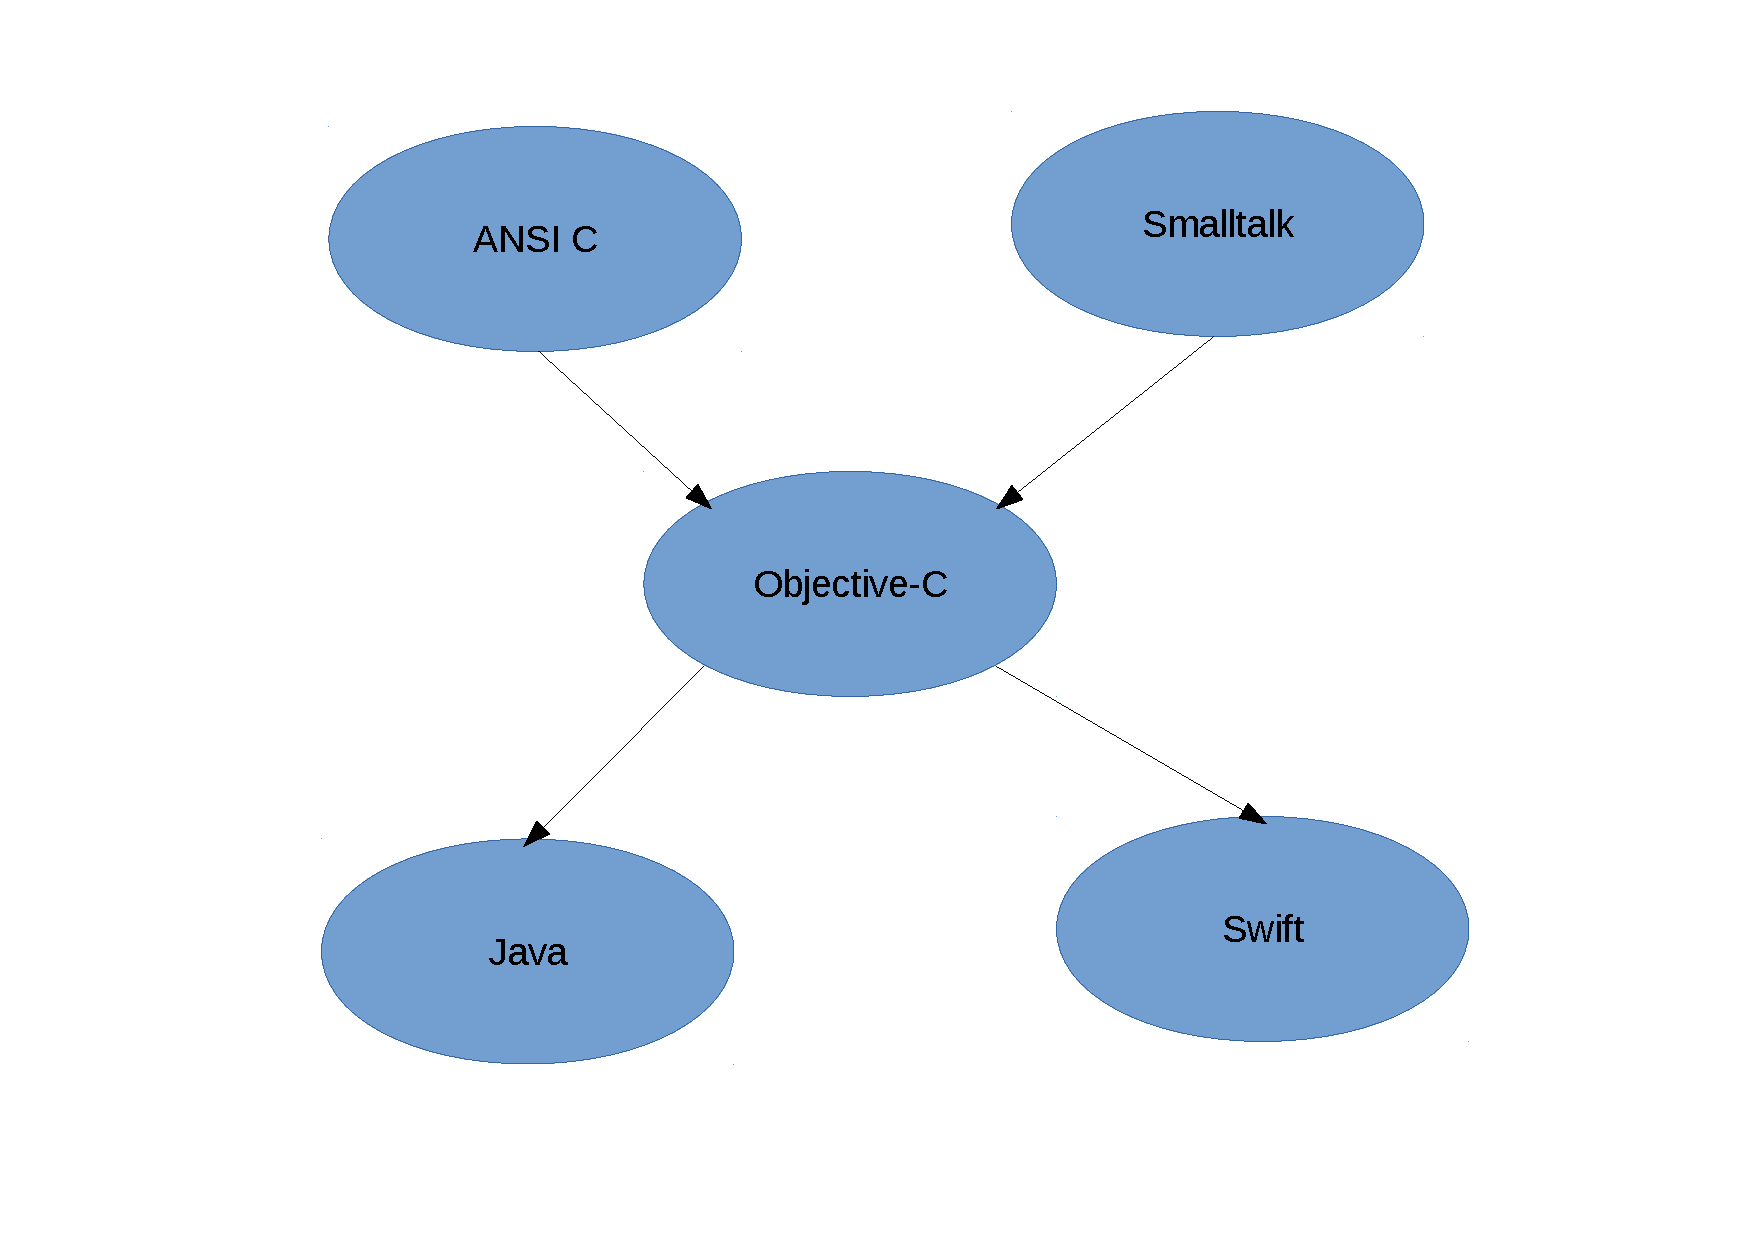
\includegraphics[scale=0.5]{razvojno_stablo}
	\caption{MVC arhitektura}	
	\label{fig:MVC}
	\end{center}
\end{figure}

\section{Eksperimentalni rezultati}

\section{Zaključak}
\label{sec:zakljucak}
U ovom radu su opisane najvažnije osobine i koncepti jezika. Objective-C predstavlja osnovu operativnih sistema koji su u širokoj upotrebi i kao takav će i u budućnosti zauzimati zapaženo mesto u svetu informatike. Trajanje (skoro 40 godina) svedoči o kvalitetu jezika. Rad prestavlja podstrek za dalje istraživanje mogućnosti i funkcionalnosti jezika i njegovih okruženja.  
\addcontentsline{toc}{section}{Literatura}
\appendix
\bibliography{DenisAlicicPSOClustering} 
\bibliographystyle{plain}
\end{document}